% !TeX root = RJwrapper.tex
\title{A Fast and Scalable Implementation Method for Competing Risks Data with the R Package \CRANpkg{fastcmprsk}}
\author{by Eric S. Kawaguchi, Jenny I. Shen, Gang Li, and Marc A. Suchard}

\maketitle

\abstract{
Advancements in medical informatics tools and high-throughput biological experimentation make large-scale biomedical data routinely accessible to researchers. Competing risks data are typical in biomedical studies where individuals are at risk to more than one cause (type of event) which can preclude the others from happening. The \cite{fine1999proportional} is a popular and well-appreciated model for competing risks data and is currently implemented in a number of statistical software packages. However, current implementations are not computationally scalable for large-scale competing risks data. We have developed an R package, \CRANpkg{fastcmprsk}, that uses a novel forward-backward scan algorithm to significantly reduce the computational complexity for parameter estimation by exploiting the structure of the subject-specific risk sets. Numerical studies compare the speed and scalability of our implementation to current methods for unpenalized and penalized Fine-Gray regression and show impressive gains in computational efficiency.}

\section{Introduction} 

\label{sec3:intro}
Competing risks time-to-event data arise frequently in biomedical research when subjects are at risk for more than one type of possibly correlated events or causes and the occurrence of one event precludes the others from happening. 
For example, one may wish to study time until first kidney transplant for kidney dialysis patients with end state renal disease. Then
terminating events such as death, renal function recovery, or discontinuation of dialysis are competing risks as their occurrence will prevent subjects from receiving a transplant.  When modeling competing risks data the cumulative incidence function (CIF), the probability of observing a certain cause while taking the other causes (known as the competing risks) into account, is oftentimes a quantity of interest. 

The most commonly-used model to draw inference about the covariate effect on the CIF and to predict the CIF dependent on a set of covariates is the Fine-Gray proportional subdistribution hazards model \citep{fine1999proportional}. Various statistical packages for estimating the parameters of the Fine-Gray model are popular within the {R} programming language \citep{ihaka1996}. One package, among others, is the \CRANpkg{cmprsk} \citep{cmprsk} package. The \CRANpkg{riskRegression} \citep{riskRegression} package, initially implemented for predicting absolute risks \citep{gerds2012absolute}, uses a wrapper that calls the \CRANpkg{cmprsk} package to perform Fine-Gray regression. \cite{scheike2011analyzing} provide \CRANpkg{timereg} \citep{timereg} that allows for general modeling of the cumulative incidence function and includes the Fine-Gray model as a special case. The \CRANpkg{survival} package also performs Fine-Gray regression but does so using a weighted Cox \citep{cox1972regression} model. Over the past decade, there have been several extensions to the Fine-Gray method that also result in useful packages. The \CRANpkg{crrSC} \citep{crrSC} package allows for the modeling of both stratified \citep{zhou2011competing} and clustered \citep{zhou2012competing} competing risks data. \cite{kuk2013model} propose a  stepwise Fine-Gray selection procedure and develop the \CRANpkg{crrstep} \citep{crrstep} package for implementation. \cite{fu2017penalized} then introduce penalized Fine-Gray regression with the corresponding \CRANpkg{crrp} \citep{crrp} package. 

A contributing factor to the computational complexity for general Fine-Gray regression implementation is parameter estimation. Generally, one needs to compute the log-pseudo likelihood and its first and second derivatives with respect to its regression parameters for optimization. Calculating these quantities is typically of order $O(n^2)$, where $n$ is the number of observations in the dataset, due to the repeated calculation of the subject-specific risk sets. With current technological advancements making large-scale data from  electronic health record (EHR) data systems routinely accessible to researchers, these implementations quickly become inoperable or grind-to-a-halt in this domain. For time-to-event data with no competing risks \cite{mittal2013high}, among others, have made significant progress in reducing the computational complexity for the Cox proportional hazards model from $O(n^2)$ to $O(n)$ by taking advantage of the cumulative structure of the risk set. However, the counterfactual construction of the risk set for the Fine-Gray model does not retain the same structure and presents a barrier to reducing the complexity of the risk set calculation. To the best of our knowledge, no further advancements in reducing the computational complexity required for calculating the subject-specific risk sets exists. 

The contribution of this work is the development of an {R} package \CRANpkg{fastcmprsk} \citep{fastcmprsk}  which implements a novel forward-backward scan algorithm \citep{kawaguchi2019scalable} for the Fine-Gray model. By taking advantage of the ordering of the data and the structure of the risk set, we can calculate the log-pseudo likelihood and its derivatives, which are necessary for parameters estimation, in $O(n)$ time rather than $O(n^2)$. As a consequence, our approach is scalable to large competing risks datasets and outperforms competing algorithms for both penalized and unpenalized parameter estimation. 

The paper is organized as follows. In the next section, we briefly review the basic definition of the Fine-Gray proportional subdistribution hazards model, the CIF, and penalized Fine-Gray regression. We introduce our forward-backward scan algorithm in Section \ref{s3:scan}. Then, in Section \ref{s3:pkg} we describe the main functionalities of the \CRANpkg{fastcmprsk} package that we developed for {R} which utilizes the aforementioned algorithm, which include unpenalized and penalized parameter estimation and CIF estimation. We perform simulation studies in Section \ref{s3:sim} to compare the performance of our proposed method to some of their popular competitors. The \CRANpkg{fastcmprsk} package is readily available on the Comprehensive R Archive Network (CRAN) at \url{https://CRAN.R-project.org/package=fastcmprsk}.
%% -- Manuscript ---------------------------------------------------------------

%% - In principle "as usual" again.
%% - When using equations (e.g., {equation}, {eqnarray}, {align}, etc.
%%   avoid empty lines before and after the equation (which would signal a new
%%   paragraph.
%% - When describing longer chunks of code that are _not_ meant for execution
%%   (e.g., a function synopsis or list of arguments), the environment {Code}
%%   is recommended. Alternatively, a plain {verbatim} can also be used.
%%   (For executed code see the next section.)

\section{Preliminaries}
\subsection{Data structure and model}
\label{s3:estimator}
We first establish some notation and the formal definition of the data generating process for competing risks. 
For subject $i = 1, \ldots, n$, let $T_i$, $C_i$, and $\ep_i$ be the event time, possible right-censoring time, and cause (event type), respectively. Without loss of generality assume there are two event types $\ep \in \{1, 2\}$ where $\ep = 1$ is the event of interest (or primary event) and $\ep = 2$ is the competing risk. With the presence of right-censoring, we generally observe $X_i = T_i \mmin C_i$, $\delta_i = I(T_i \leq C_i)$, where $a \mmin b = \min(a, b)$ and $I(\cdot)$ is the indicator function. Letting $\mathbf{z}_i$ be a $p$-dimensional vector of time-independent subject-specific covariates, competing risks data consist of the following independent and identically distributed quadruplets $\{(X_i, \delta_i, \delta_i \ep_i, \mathbf{z}_i)\}_{i=1}^n$. Assume that there also exists a $\tau$ such that  1) for some arbitrary time $t$, $t \in [0, \tau]$ ; 2) $\Pr(T_i > \tau) > 0$ and $\Pr(C_i > \tau) >0$  for all $i = 1,\ldots, n$, and that for simplicity, no ties are observed.

The CIF for the primary event  conditional on the covariates $\mathbf{z} = (z_1, \ldots, z_p)$ is $F_1(t; \mathbf{z}) = \Pr(T \leq t, \epsilon = 1|\mathbf{z})$.  To model the covariate effects on $F_1(t; \mathbf{z})$, \cite{fine1999proportional} introduced the now well-appreciated proportional subdistribution hazards (PSH) model: 
\begin{align}
\label{eq3:pshmodel}
h_1(t| \mathbf{z}) = h_{10}(t) \exp(\mathbf{z}^\prime\bbeta),
\end{align}
where \begin{align*}
h_1(t| \mathbf{z}) & =  \lim_{\Delta t \to 0} \frac{\Pr\{t \leq T \leq t + \Delta t, \epsilon = 1 | T \geq t \cup (T \leq t \cap \epsilon \neq 1), \mathbf{z}\}}{\Delta t} %\\
%& = \{d F_1(t; \mathbf{z}) / dt\} / \{1 - F_1(t; \mathbf{z})\} \\
%& 
\\&  = -\frac{d}{dt} \log\{1 - F_1(t; \mathbf{z})\}
\end{align*}
is a subdistribution hazard \citep{gray1988class}, 
$h_{10}(t)$ is a completely unspecified baseline subdistribution hazard, and $\bbeta$ is a $p \times 1$ vector of regression coefficients. 
As \cite{fine1999proportional} mentioned, the risk set associated with $h_1(t; \mathbf{z})$ is somewhat 
unnatural as it includes subjects who are still at risk $(T \geq t)$ and those who have already observed the competing risk prior to time $t$ ($T \leq t \cap \epsilon \neq 1$). However, this construction is useful  for direct modeling of the CIF.

\subsection{Parameter estimation for unpenalized Fine-Gray regression}
Parameter estimation and large-sample inference of the PSH model follows from the log-pseudo likelihood:
\begin{align}
\label{eq3:lpp}
l(\bbeta) = \sum_{i=1}^n  \int_0^\infty \left[ \mathbf{z}_i^\prime \bbeta - \ln \left\{ \sum_k \hat{w}_k(u) Y_k(u) \exp \left(\mathbf{z}_k^\prime \bbeta \right) \right\} \right] \hat{w}_i(u)dN_i(u),
\end{align}
where $N_i(t) = I(X_i \leq t, \ep_i = 1)$, $Y_i(t) = 1 - N_i(t-)$, and $\hat{w}_i(t)$ is a time-dependent weight based on the inverse probability of censoring weighting (IPCW) technique \citep{robins1992recovery}. To parallel \cite{fine1999proportional}, we define the  IPCW for subject $i$ at time $t$ as $\hat{w}_i(t) = I(C_i \geq T_i \mmin t)\hat{G}(t)/\hat{G}(X_i \mmin t)$, where $G(t) = \Pr(C \geq t)$ is the survival function of the censoring variable $C$ and $\hat{G}(t)$ is the Kaplan-Meier estimate for $G(t)$. However, we can generalize the IPCW to allow for dependence between $C$ and $\mathbf{z}$.

Let $\hat{\bbeta}_{mple} = \arg \min_{\bbeta} \{-l(\bbeta)\}$ be the maximum pseudo likelihood estimator of $\bbeta$. \cite{fine1999proportional} investigate the large-sample properties of $\hat{\bbeta}_{mple}$ and prove that, under certain regularity conditions, 
\begin{align}
\sqrt{n}(\hat{\bbeta}_{mple} - \bbeta_0) \to N(0, \Omega^{-1} \Sigma \Omega^{-1}),
\end{align}
where $\bbeta_0$ is the true value of $\bbeta$, $\Omega$ is the limit of the negative of the partial derivative matrix of the score function evaluated at $\bbeta_0$, and $\Sigma$ is the variance-covariance matrix of the limiting distribution of the score function. The package \CRANpkg{cmprsk} implements this estimation procedure. 

\subsection{Estimating the cumulative incidence function}
An alternative interpretation of the coefficients from the Fine-Gray model is to model their effect on the CIF. Using a Breslow-type estimator \citep{breslow1974covariance}, we can obtain a consistent estimate for $H_{10}(t) = \int_0^t h_{10}(s)ds$ through
\begin{align*}
\hat{H}_{10}(t) = \frac{1}{n} \sum_{i=1}^n \int_0^t \frac{1}{\hat{S}^{(0)}(\hat{\bbeta}, u)}\hat{w}_i(u)dN_i(u),
\end{align*}
where $\hat{S}^{(0)}(\hat{\bbeta}, u) = n^{-1} \sum_{i=1}^n \hat{w}_i(u)Y_i(u)\exp(\mathbf{z}_i^\prime\hat{\bbeta})$.
The predicted CIF, conditional on $\mathbf{z} = \mathbf{z}_0$, is then
\begin{align*}
\hat{F}_1(t;\mathbf{z}_0) = 1 - \exp\left\{\int_0^t \exp(\mathbf{z}^\prime_0 \hat{\bbeta})d\hat{H}_{10}(u)\right\}.
\end{align*}
We refer the readers to Appendix B of \cite{fine1999proportional} for the large-sample properties of $\hat{F}_1(t; \mathbf{z}_0)$. The quantities needed to estimate $\int_0^t d\hat{H}_{10}(u)$ are already precomputed when estimating $\hat{\bbeta}$. \cite{fine1999proportional} proposed a resampling approach to calculate confidence intervals and confidence bands for $\hat{F}_1(t; \mathbf{z}_0)$.
 

\subsection{Penalized Fine-Gray regression for variable selection}
\label{s3:pen}
%Our method to speed up the parameter estimation for the Fine-Gray model can be adapted to several applications \citep{zhou2011competing, zhou2012competing, fu2017penalized}. We extend our approach for linearized estimation to penalized Fine-Gray regression. 

Oftentimes, reserachers are interested in identifying which covariates have an effect on the CIF. Penalization methods  \citep{tibshirani1996regression, fan2001variable, zou2006adaptive, zhang2010regularization} offer a popular way to perform variable selection and parameter estimation simultaneously through minimizing the objective function
\begin{align}
Q(\bbeta) = -l(\bbeta) + \sum_{j=1}^p p_\lambda(|\beta_j|),
\end{align}
where $l(\bbeta)$ is defined in (\ref{eq3:lpp}), $p_{\lambda}(|\beta_j|)$ is a penalty function where the sparsity of the model is controlled by the non-negative tuning parameter $\lambda$. \cite{fu2017penalized} recently extend several popular variable selection procedures - LASSO \citep{tibshirani1996regression}, SCAD \citep{fan2001variable}, adaptive LASSO \citep{zou2006adaptive}, and MCP \citep{zhang2010nearly} - to the Fine-Gray model, explore its asymptotic properties under fixed model dimension, and develop the {R} package \CRANpkg{crrp} \citep{crrp} for implementation. Parameter estimation in the \CRANpkg{crrp} package employs a cyclic coordinate algorithm.

The sparsity of the model depends heavily on the choice of the tuning parameters. Practically, finding a suitable (or optimal) tuning parameter involves applying a penalization method over a sequence of possible candidate values of $\lambda$ and finding the $\lambda$ that minimizes some metric such as the Bayesian information criterion \citep{schwarz1978estimating} or generalized cross validation measure \citep{craven1978smoothing}. A more thorough discussion on tuning parameter selection can partially be found in 
 \cite{wang2007tuning, zhang2010regularization, wang2011consistent,  fan2013tuning, fu2017penalized, ni2018tuning}.

 \section{Forward-backward scan for parameter estimation}
 \label{s3:scan}
 This section discusses a novel forward-backward scan algorithm, proposed in \cite{kawaguchi2019scalable}, that reduces the computational complexity associated with parameter estimation from $O(n^2)$ to $O(n)$. Commonly-used optimization routines generally require the calculation of the log-pseudo likelihood (\ref{eq3:lpp}), the score function
 \begin{align}
\label{eq3:psh_score}
\dot{l}_j(\bbeta) = & \sum_{i=1}^n I(\delta_i\ep_i = 1) z_{ij} - \sum_{i = 1}^n I(\delta_i\ep_i = 1) \frac{ \sum_{k \in R_i} z_{kj} \tilde{w}_{ik}  \exp(\eta_k)}{\sum_{k \in R_i} \tilde{w}_{ik} \exp(\eta_k)}, 
\end{align}
and, in some cases, the Hessian digonals
\begin{align}
\label{eq3:psh_hess}
\ddot{l}_{jj}(\bbeta) = & \sum_{i=1}^n I(\delta_i\ep_i = 1) \left[ \frac{ \sum_{k \in R_i} z_{kj}^2 \tilde{w}_{ik}  \exp(\eta_k)}{\sum_{k \in R_i} \tilde{w}_{ik} \exp(\eta_k)} -  \left\{ \frac{ \sum_{k \in R_i} z_{kj} \tilde{w}_{ik}  \exp(\eta_k)}{\sum_{k \in R_i} \tilde{w}_{ik} \exp(\eta_k)} \right\}^2 \right], 
\end{align}
where  $$\tilde{w}_{ik} = \hat{w}_k(X_i) = \hat{G}(X_i) / \hat{G}(X_i \mmin X_k), \quad k \in R_i,$$ 
$R_i = \{y:(X_y \geq X_i) \cup (X_y \leq X_i \cap \epsilon_y =  2)\}$ and
$\eta_k = \mathbf{z}_k^\prime\bbeta$ for use within cyclic coordinate descent. {\color{blue} Despite $\eta$ and $\hat{G}(X)$ being fixed quantities within the calculation of (\ref{eq3:lpp}), (\ref{eq3:psh_score}), and (\ref{eq3:psh_hess}), directly evaluating these quantities using the above formulas will require $O(n^2)$ operations due to the structure of the risk set within the double summation, and will be computationally taxing for large $n$.} Below we will show how to calculate the double summation linearly using a forward-backward scan algorithm, that allows us to compute (\ref{eq3:lpp}), (\ref{eq3:psh_score}), and (\ref{eq3:psh_hess}) in $O(n)$ time.

Before proceeding with the algorithm, we first define what we mean by a forward and backward scan. A forward (prefix) scan maps $\{a_1, a_2, \ldots, a_n\} \mapsto \{a_1, a_1 + a_2, \ldots, \sum_{i=1}^n a_i\}$; whereas a backward (prefix) scan maps to $\{\sum_{i=1}^n a_i, \sum_{i=2}^n a_i, \ldots, a_1\}$. 
First, note that $R_i$ partitions into two disjoint subsets: $R_i(1) = \{y:X_y \geq X_i\}$ and $R_i(2) = \{y:(X_y \leq X_i \cap \epsilon_y =  2) \}$. Here $R_i(1)$ is the set of observations that have an observed event time after $X_i$ and $R_i(2)$ is the set of observations that have observed the competing event before time $X_i$. Further, $\tilde{w}_{ik} = 1$ if $k \in R_i(1)$ and $\tilde{w}_{ik} = \hat{G}(X_i) / \hat{G}(X_k),$ if $k \in R_i(2)$. Since $R_i(1)$ and $R_i(2)$ are disjoint, we can write the double summation of, for example, the score function (\ref{eq3:psh_score}) as
\begin{align}
\label{eq3:psh_score2}
\sum_{i = 1}^n I(\delta_i\ep_i = 1) \frac{ \sum_{k \in R_i(1)} z_{kj} \exp(\eta_k) +   \hat{G}(X_i)\sum_{k \in R_i(2)} z_{kj} \exp(\eta_k) / \hat{G}(X_k)}{\sum_{k \in R_i(1)} \exp(\eta_k) +  \hat{G}(X_i) \sum_{k \in R_i(2)} \exp(\eta_k) / \hat{G}(X_k)}. 
\end{align}
We will first tackle the denominator term $\sum_{k \in R_i(1)} \exp(\eta_k) +  \hat{G}(X_i) \sum_{k \in R_i(2)} \exp(\eta_k) / \hat{G}(X_k)$.
If we arrange the observed event times in decreasing order, we see that  $\sum_{k \in R_i(1)} \exp(\eta_k)$ is a series of cumulative sums. For example, given $X_i > X_{i'}$, the set $R_{i'}(1)$  consists of the observations from $R_i(1)$ and  the set of observations $\{y: X_y \in [X_{i'}, X_{i})\}$, therefore $\sum_{k \in R_{i'}(1)} \exp(\eta_k) = \sum_{k \in R_i(1)}  \exp(\eta_k) + \sum_{k \in \{y: X_y \in [X_{i'}, X_{i})\}} \exp(\eta_k)$ and  thus calculating $\sum_{k \in R_i(1)} \exp(\eta_k)$ for all $i = 1, \ldots, n$ requires $O(n)$ calculations in total. However, $ \hat{G}(X_i) \sum_{k \in R_i(2)} \exp(\eta_k) / \hat{G}(X_k)$ does not monotonically increase as the event times decrease. Instead, we observe that $ \hat{G}(X_i) \sum_{k \in R_i(2)} \exp(\eta_k) / \hat{G}(X_k)$  is a series of cumulative sums as the event times increase. Thus calculating the denominator term will requires two scans: one forward scan going forward from largest observed event time to smallest to calculate $\sum_{k \in R_i(1)} \exp(\eta_k) $ and one backward scan from smallest observed event time to largest to calculate $ \hat{G}(X_i) \sum_{k \in R_i(2)} \exp(\eta_k) / \hat{G}(X_k)$. Likewise, we calculate both $\sum_{k \in R_i} z_{kj} \exp(\eta_k)$ and $\sum_{k \in R_i} z_{kj}^2 \exp(\eta_k)$ in linear time since the terms $z_{kj}$ and $z_{kj}^2$ are multiplicative constants that do not affect the cumulative structures of the summations. As a consequence, the ratio in the double summation is available in $O(n)$ time.

Furthermore, the outer summation of subjects who observe the event of interest is also a cumulative sum since, provided that $X_i > X_{i'}$ and both $\delta_i = 1$ and $\delta_{i'} = 1$,
\begin{align}
\sum_{l = 1}^{i} I(\delta_{l} \ep_l = 1) \frac{ \sum_{k \in R_l} z_{kj} \exp(\eta_k)}{\sum_{k \in R_l} \exp(\eta_k)} & = \sum_{l = 1}^{i'} I(\delta_{l}\ep_l = 1) \frac{ \sum_{k \in R_l} z_{kj} \exp(\eta_k)}{\sum_{k \in R_l} \exp(\eta_k)} \\
&  + I(\delta_{i}\ep_i = 1) \frac{ \sum_{k \in R_{i}} z_{kj} \exp(\eta_k)}{\sum_{k \in R_{i}} \exp(\eta_k)} , 
\end{align}
that also only requires $O(n)$ calculations since the ratios are precomputed in $O(n)$ calculations and thus the score function (\ref{eq3:psh_score}) can be calculated in linear time. Similarly, both the log-pseudo likelihood (\ref{eq3:lpp}) and the diagonal elements of the Hessian (\ref{eq3:psh_hess}) are also calculated linearly. We refer readers to \cite{kawaguchi2019scalable} for a thorough disucssion.

\section{The fastcmprsk package}
\label{s3:pkg}
We utilize this forward-backward scan algorithm for both penalized and unpenalized parameter estimation for the  Fine-Gray model in linear time. Furthermore, we also develop scalable methods to estimate the predicted CIF and its corresponding confidence interval/band. For convenience to researchers and readers, we further include a function to simulate two-cause competing risks data. Table 1 provides a quick summary of the currently available functions provided in \CRANpkg{fastcmprsk}. We briefly detail the use of these functions below.

\begin{table}[t]
\centering
\begin{tabular}{ll}
  \toprule
  Function name & Basic description \\
  \hline
  \em{Modeling functions} & \\
  \code{fastCrr}  & Fits unpenalized Fine-Gray regression \\
  \code{fastCrrp} & Fits penalized Fine-Gray regression\\
  \midrule
  \em{Utilities} & \\
  %\code{summary} & Returns ANOVA table from \code{fastCrr} output \\
  %\code{predict} & Estimates CIF given a vector of covariates \\
  %\code{plot} &  Plots output (object dependent) \\
  \code{varianceControl } & Options for bootstrap variance\\
  \code{simulateTwoCauseFineGrayModel} & Simulates two-cause competing risks data\\
   \bottomrule
\end{tabular}
\label{tab3:list}
\caption{Currently available functions in \CRANpkg{fastcmprsk}.}
\end{table}

\subsection{Simulating competing risks data}
Researchers can simulate two-cause competing risks data using the \code{simulateTwoCauseFineGrayModel} function in \CRANpkg{fastcmprsk}. The data generation scheme follows a similar design to that of \cite{fine1999proportional} and \cite{fu2017penalized}. Given a design matrix $\mathbf{Z} = (\mathbf{z}_1^\prime, \ldots, \mathbf{z}_n^\prime)$, $\bbeta_1$, and $\bbeta_2$, let the cumulative incidence function for cause 1 (the event of interest) be defined as
$F_1(t; \mathbf{z}_i) = \Pr(T_i \leq t, \epsilon_i = 1|\mathbf{z}_i) = 1 - [1 - \pi\{1-\exp(-t)\}]^{\exp(\mathbf{z}_i^\prime\bbeta_1)}$,
which is a unit exponential mixture with mass $1 - \pi$ at $\infty$ when $\mathbf{z}_i = \mathbf{0}$ and where $\pi$ controls the cause 1 event rate. The cumulative incidence function for cause 2 is obtained by setting 
$\Pr(\epsilon_i = 2 | \mathbf{z}_i) = 1 - \Pr(\epsilon_i = 1|\mathbf{z}_i)$ and then using an exponential distribution with rate $\exp(\mathbf{z}^\prime_i\bbeta_2)$ for the conditional cumulative incidence function $\Pr(T_i \leq t|\epsilon_i = 2, \mathbf{z}_i)$. Censoring times are independently generated from a uniform distribution $U(u\mbox{\tiny{min}}, u\mbox{\tiny{max}})$ where $u\mbox{\tiny{min}}$ and $u\mbox{\tiny{max}}$ control the censoring percentage. Appendix \ref{app3:data} provides more details on the data generation process.  Below is a toy example of simulating competing risks data where $n = 500$, $\bbeta_1  = (0.40, -0.40, 0, -0.50, 0, 0.60, 0.75, 0, 0, -0.80)$, $\bbeta_2  =-\bbeta_1$, $u\mbox{\tiny{min}} = 0$, $u\mbox{\tiny{max}} = 1$, $\pi = 0.5$, and where $\mathbf{Z}$ is simulated from a multivariate standard normal distribution with unit variance. This simulated dataset will be used to illustrate the use of the different modeling functions within \CRANpkg{fastcmprsk}.


\begin{example}
R> library(fastcmprsk)
R> set.seed(2019)
R> nobs <- 500
R> beta1 <- c(0.40, -0.40,  0, -0.50,  0,  0.60,  0.75,  0,  0, -0.80)
R> beta2 <- -beta1
R> Z <- matrix(rnorm(nobs * length(beta1)), nrow = nobs)
R> dat <- simulateTwoCauseFineGrayModel(nobs, beta1, beta2, 
+	Z, u.min = 0, u.max = 1, p = 0.5)
R> table(dat$fstatus) # Event counts

  0   1   2 
241 118 141 

head(dat$ftime) # First 6 observed survival times

[1] 0.098345608 0.008722629 0.208321175 0.017656904 0.495185038 0.222799124
\end{example}


\subsection{Unpenalized parameter estimation and inference}
We first illustrate the coefficient estimation from (\ref{eq3:pshmodel}) using the Fine-Gray log-pseudo likelihood. 
The \code{fastCrr} function estimates these parameters using our forward-backward scan algorithm and is syntactically similar to the \code{coxph} function in \CRANpkg{survival}. The \code{formula} argument requires a newly-defined \code{Crisk} object as an outcome. The \code{Crisk} function produces a \code{Crisk} object by calling the \code{Surv} function in \CRANpkg{survival}, modifying it to allow for more than one event, and requires four arguments: a vector of observed event times (\code{ftime}), a vector of corresponding event/censoring indicators (\code{fstatus}), the value of \code{fstatus} that denotes a right-censored observation (\code{cencode}) and the value of \code{fstatus} that denotes the event of interest (\code{failcode}). By default, \code{Crisk} assumes that \code{cencode = 0} and \code{failcode = 1}.
\begin{example}
# cmprsk package
R> fit1 <- crr(dat$ftime, dat$fstatus, Z, failcode = 1, cencode = 0,
+                      variance = FALSE)

# fastcmprsk package
R> fit2 <- fastCrr(Crisk(dat$ftime, dat$fstatus, cencode = 0, failcode = 1) ~ Z,
+                           variance = FALSE,
+                           returnDataFrame = TRUE)

R> max(abs(fit1$coef - fit2$coef))
\end{example}
\begin{example}
[1] 8.534242e-08
\end{example}
As expected, the \code{fastCrr} function calculates nearly identical parameter estimates to the \code{crr} function. We compare the runtime performance between these two methods in Section \ref{s3:crr}.

We now show how to obtain the variance-covariance matrix for the parameter estimates. The variance-covariance matrix for $\hat{\bbeta}$ can not be directly estimated using the \code{fastCrr} function. First, the asymptotic expression requires estimating both $\Omega$ and $\Sigma$, which can not be trivially calculated in linear time. Second, for large-scale data where both $n$ and $p$ can be large, matrix calculations, storage, and inversion can be computationally prohibitive. Instead, we propose to estimate the variance-covariance matrix using the bootstrap \citep{efron1979bootstrap}.  Let $\tilde{\bbeta}^{(1)}, \ldots \tilde{\bbeta}^{(B)}$ be bootstrapped parameter estimates obtained by resampling subjects with replacement from the original data $B$ times. Unless otherwise noted, the size of each resample is the same as the original data. For $j = 1, \ldots, p$ and $k = 1, \ldots, p$, we can estimate the covariance between $\hat{\beta}_j$ and $\hat{\beta}_k$ by
 \begin{align}
\widehat{Cov}(\hat{\beta}_j, \hat{\beta}_k) = \frac{1}{B - 1} \sum_{b = 1}^B (\tilde{\beta}^{(b)}_{j} - \bar{\beta}_j)(\tilde{\beta}^{(b)}_{k} - \bar{\beta}_k),
\end{align}
where $\bar{\bbeta}_j = \frac{1}{B} \sum_{b=1}^B \tilde{\bbeta}^{(b)}_{j}$. Therefore, with $\hat{\sigma}^2_j = \widehat{Cov}(\hat{\beta}_j, \hat{\beta}_j$), a $(1 - \alpha) \times 100\%$ confidence interval for $\bbeta_j$ is given by
\begin{align}
\hat{\beta}_j \pm z_{1-\alpha/2} \hat{\sigma}_j,
\end{align}
where $z_{1 - \alpha / 2}$ is the $(1 - \alpha) \times 100th$ percentile of the standard normal distribution. Since parameter estimation for the Fine-Gray model can be done in linear time using our forward-backward scan algorithm, the collection of parameter estimates obtained by bootstrapping can also be obtained linearly. The \code{varianceControl} function controls the parameters used for bootstrapping, that one then passes into the \code{var.control} argument in \code{fastCrr}.
\begin{example}
R> vc   <- varianceControl(B = 100, seed = 2019)
R> fit3 <- fastcmprsk::fastCrr(Crisk(dat$ftime, dat$fstatus) ~ Z, variance = TRUE,
+                              var.control = vc,
+                              returnDataFrame = TRUE)
# returnDataFrame = TRUE is necessary for CIF estimation (next section)

R> round(sqrt(diag(fit3$var)), 3)
\end{example}
\begin{example}
 [1] 0.108 0.123 0.085 0.104 0.106 0.126 0.097 0.097 0.104 0.129
\end{example}
\begin{example}
R> summary(fit3, conf.int = FALSE, digits = 2)
\end{example}
\begin{example}
Fine-Gray Regression via fastcmprsk package. 

fastCrr converged in 24 iterations.
 
Call:
fastcmprsk::fastCrr(Crisk(dat$ftime, dat$fstatus) ~ Z, variance = TRUE, 
    var.control = vc, returnDataFrame = TRUE)

        coef exp(coef) se(coef) z value Pr(>|z|)
x1   0.19228     1.212   0.1081   1.779 7.52e-02
x2  -0.38640     0.679   0.1227  -3.149 1.64e-03
x3   0.01816     1.018   0.0854   0.213 8.32e-01
x4  -0.39769     0.672   0.1042  -3.816 1.36e-04
x5   0.10571     1.111   0.1060   0.997 3.19e-01
x6   0.57494     1.777   0.1259   4.568 4.92e-06
x7   0.77884     2.179   0.0974   7.998 1.33e-15
x8  -0.00611     0.994   0.0969  -0.063 9.50e-01
x9  -0.06571     0.936   0.1042  -0.631 5.28e-01
x10 -0.99687     0.369   0.1286  -7.750 9.10e-15

Pseudo Log-likelihood = -590 
Null Pseudo Log-likelihood = -675 
Pseudo likelihood ratio test = 170 on 10 df. 
\end{example}

{\color{blue}
Since standard error estimation is performed via bootstrap and resampling, it is easy to use multiple cores to speed up computation. Parallelization is seamlessly implemented using the \CRANpkg{doParallel} package \citep{doParallel}. Enabling usage of multiple cores is done through the \code{useMultipleCores} argument within the \code{varianceControl} function. To avoid interference with other processes, we allow users to set up the cluster on their own. We provide an example below.

\begin{example}
R> library(doParallel) 

R> n.cores <- 2 # No. of cores
R> myClust <- makeCluster(n.cores)

R> vc = varianceControl(B = 1000, useMultipleCores = TRUE)

R> registerDoParallel(myClust)
R> system.time(
R> fit3 <- fastCrr(Crisk(dat$ftime, dat$fstatus) ~ Z, variance = TRUE,
+                             var.control = vc,
+                             returnDataFrame = TRUE)
+ )
R> stopCluster(myClust)
\end{example}
}


\subsection{Cumulative incidence function and interval/band estimation}
The CIF is also available in linear time in the \CRANpkg{fastcmprsk} package. \cite{fine1999proportional} propose a Monte Carlo simulation method for interval and band estimation. We implement a slightly different approach using bootstrapping for interval and band estimation in our package. Let $\tilde{F}^{(1)}_1(t; \mathbf{z}_0), \ldots, \tilde{F}^{(B)}_1(t; \mathbf{z}_0)$ be the bootstrapped predicted CIF obtained by resampling subjects with replacement from the original data $B$ times and let $m(\cdot)$ be a known, monotone, and continuous transformation. In our current implementation we let $m(x) = \log\{-\log(x)\}$; however, we plan on incorporating other transformations in our future implementation. We first estimate the variance function $\sigma^2(t; \mathbf{z}_0)$ of the transformed CIF through
\begin{align}
\label{eq3:boot_var_est}
\hat{\sigma}^2(t; \mathbf{z}_0) = \frac{1}{B} \sum_{b=1}^B \left[ m\{\tilde{F}^{(b)}_1(t; \mathbf{z}_0)\} - \bar{m}\{\tilde{F}_1(t; \mathbf{z}_0)\} \right]^2,
\end{align}
where $\bar{m}\{\tilde{F}_1(t; \mathbf{z}_0)\}  = \frac{1}{B} \sum_{b=1}^B m\{\tilde{F}^{(b)}_1(t; \mathbf{z}_0)\}$. Using the functional delta method, we can now construct $(1 - \alpha) \times 100\%$ confidence intervals for $F_1(t; \mathbf{z}_0)$ by 
\begin{align}
\label{eq3:boot_cif_int}
m^{-1} \left[ m\{\hat{F}_1(t; \mathbf{z}_0)\} \pm z_{1 - \alpha / 2} \hat{\sigma}(t; \mathbf{z}_0)\right].
\end{align}

Next we propose a symmetric global confidence band for the estimated CIF $\hat{F}_1(t; \mathbf{z}_0)$, $t \in [t_L, t_U]$ via bootstrap. We first determine a critical region $C_{1 - \alpha}(\mathbf{z}_0)$ such that 
\begin{align}
\Pr \left\{ \sup_{t \in [t_L, t_U]}  \frac{| m\{\hat{F}_1(t; \mathbf{z}_0)\} - m\{F_1(t; \mathbf{z}_0)\} |}{\sqrt{\widehat{Var}[m\{\hat{F}_1(t; \mathbf{z}_0)\}]}} \leq C_{1 - \alpha}(\mathbf{z}_0) \right\} = 1 - \alpha. 
\end{align}
While Equation (\ref{eq3:boot_var_est}) estimates $\widehat{Var}[m\{\hat{F}_1(t; \mathbf{z}_0)\}]$ we still need to find $C_{1 - \alpha}(\mathbf{z}_0)$ by the bootstrap $(1-\alpha)^{th}$ percentile of the distribution of the supremum in the equation above.  The algorithm is as follows:
\begin{enumerate}
\item Resample subjects with replacement from the original data $B$ times and estimate $\tilde{F}^{(b)}_1(t; \mathbf{z}_0)$ for $b = 1, \ldots, B$ and $\hat{\sigma}^2(t; \mathbf{z}_0)$ using (\ref{eq3:boot_var_est}).
\item For the $b^{th}$ bootstrap sample , $b \in \{1, \ldots, B\}$, calculate
\begin{align*}
C^{(b)} = \sup_{t \in [t_L, t_U]}  \frac{| m\{\tilde{F}^{(b)}_1(t; \mathbf{z}_0)\} - m\{\hat{F}_1(t; \mathbf{z}_0)\} |}{\hat{\sigma}(t; \mathbf{z}_0)}. 
\end{align*}
\item Estimate $C_{1 - \alpha}(\mathbf{z}_0)$ from the sample $(1 - \alpha)^{th}$ percentile of the $B$ values of $C^{(b)}$, denoted by $\hat{C}_{1 - \alpha}(\mathbf{z}_0)$.
\end{enumerate}

Finally, the $(1 - \alpha) \times 100\%$ confidence band for $F_{1}(t; \mathbf{z}_0)$, $t \in [t_L, t_U]$ is given by 
\begin{align}
\label{eq3:boot_cif_band}
m^{-1} \left[ m\{\hat{F}_1(t; \mathbf{z}_0)\} \pm \hat{C}_{1 - \alpha }(\mathbf{z}_0) \hat{\sigma}(t; \mathbf{z}_0)\right].
\end{align}
One can perform CIF estimation and interval/band estimation using the \code{predict} function.

\begin{example}
R> set.seed(2019)
R> z0 <- rnorm(10) # New covariate entries to predict
R> cif.point <- predict(fit2, newdata = z0, getBootstrapVariance = TRUE,
+                      type = "interval", tL = 0.2, tU = 0.9,
+                      var.control = varianceControl(B = 100, seed = 2019))

R> plot(cif.point)                      
\end{example}

%We would like to close this section by cautioning readers to certain scenarios where bootstrapping may perform poorly. Calculating (\ref{eq3:boot_var_est}) requires estimating the CIF, $\tilde{F}_1^{(b)}(t; \mathbf{z}_0)$, at all observed primary event times. 
%Although bootstrapping is a convenient approach for constructing confidence intervals and bands, there are instances where it may lead to poor estimation. For example, $\hat{\sigma}^2(t; \mathbf{z}_0)$ may poorly estimate $\sigma^2(t; \mathbf{z}_0)$ if the number of primary events is low. This is due to the fact that the CIF is discretely estimated and that the randomness involved in resampling may result in poor estimation of the CIF, especially toward the tails. Likewise, the specification of $t_L$ and $t_U$ may also affect band estimation and we suggest readers to calculate confidence bands over an interval where there are a large number of event times.
 
\begin{figure}[t!]
\centering
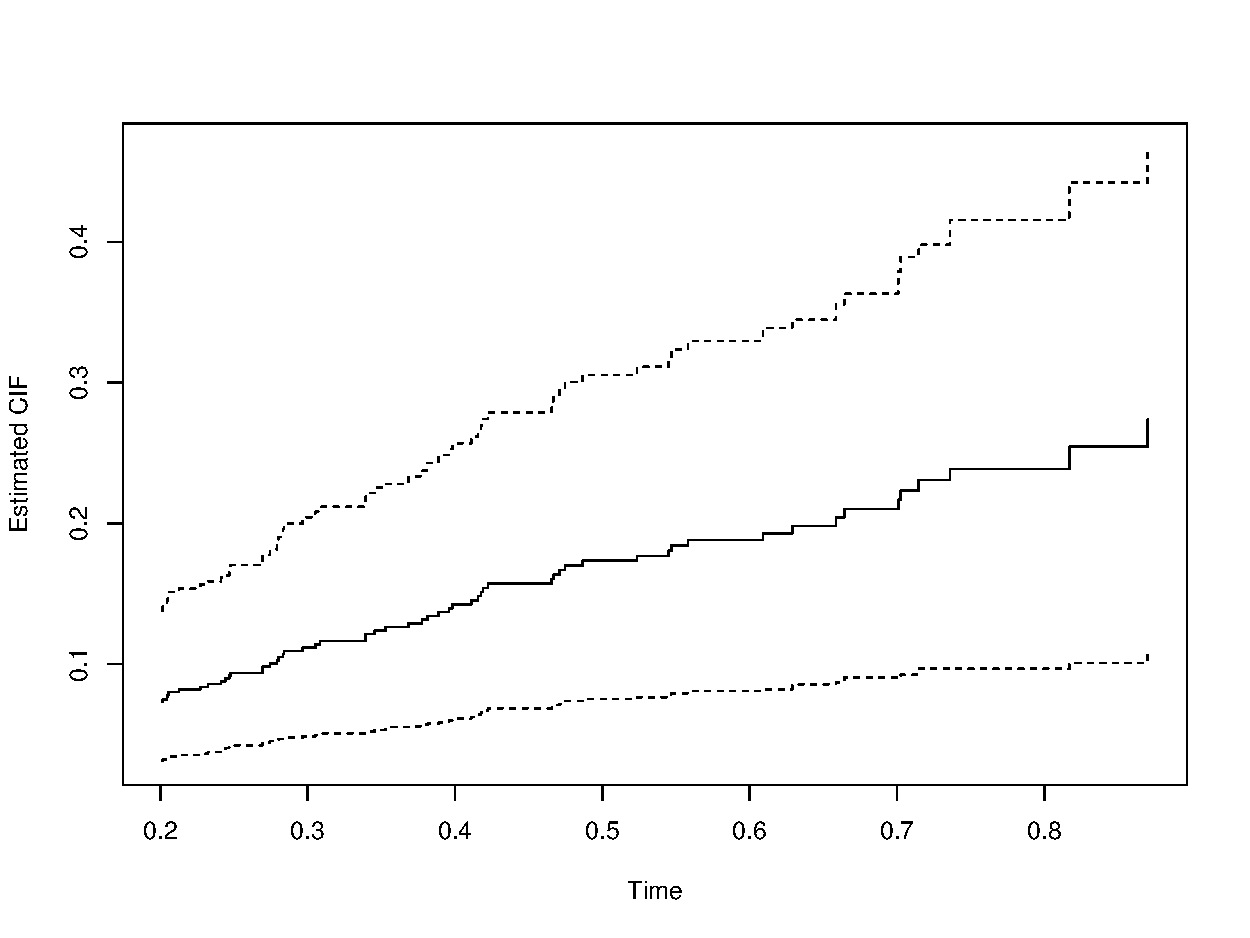
\includegraphics[scale = 0.6]{plots/new_CIF-eps-converted-to.pdf}
\label{fig2:timing}
\caption{CIF estimate and corresponding $95\%$ confidence intervals between $t_L = 0.2$ and $t_U = 0.9$.}
\end{figure}

\subsection{Penalized Fine-Gray regression via forward-backward scan}
We extend our forward-backward scan approach for for penalized Fine-Gray regression as described in Section \ref{s3:pen}.  The \code{fastCrrp} function performs LASSO, SCAD, MCP, and ridge \citep{hoerl1970ridge} penalization.  The advantage of implementing this algorithm for penalized Fine-Gray regression is two fold. Since the cyclic coordinate descent algorithm used in the \code{crrp} function calculates the gradient and Hessian diagonals in $O(pn^2)$ time, as opposed to $O(pn)$ using our approach, we expect to see drastic differences in runtime for large sample sizes. Second, as mentioned earlier, researchers generally tune the strength of regularization through multiple model fits over a grid of candidate tuning parameter values. Thus the difference in runtime between both methods grows larger as the number of candidate values increases. Below provides an example of performing LASSO-penalized Fine-Gray regression using 25 candidate values for $\lambda$. The syntax for \code{fastCrrp} is nearly identical to the syntax for \code{crrp}. 
\begin{example}
R> library(crrp)
R> lam.path <- 10^seq(log10(0.1), log10(0.001), length = 25)

R> # crrp package
R> fit.crrp <- crrp(dat$ftime, dat$fstatus, Z, penalty = "LASSO",
+                         lambda = lam.path, eps = 1E-6)

R> # fastcmprsk package
R> fit.fcrrp <- fastCrrp(Crisk(dat$ftime, dat$fstatus) ~ Z, penalty = "LASSO",
+                                    lambda = lam.path)


R> max(abs(fit.fcrrp$coef - fit.crrp$beta))
\end{example}
\begin{example}
[1] 1.110223e-15
\end{example}
\begin{example}
R> plot(fit.fcrrp) # Figure 2
\end{example}

\begin{figure}[t!]
\centering
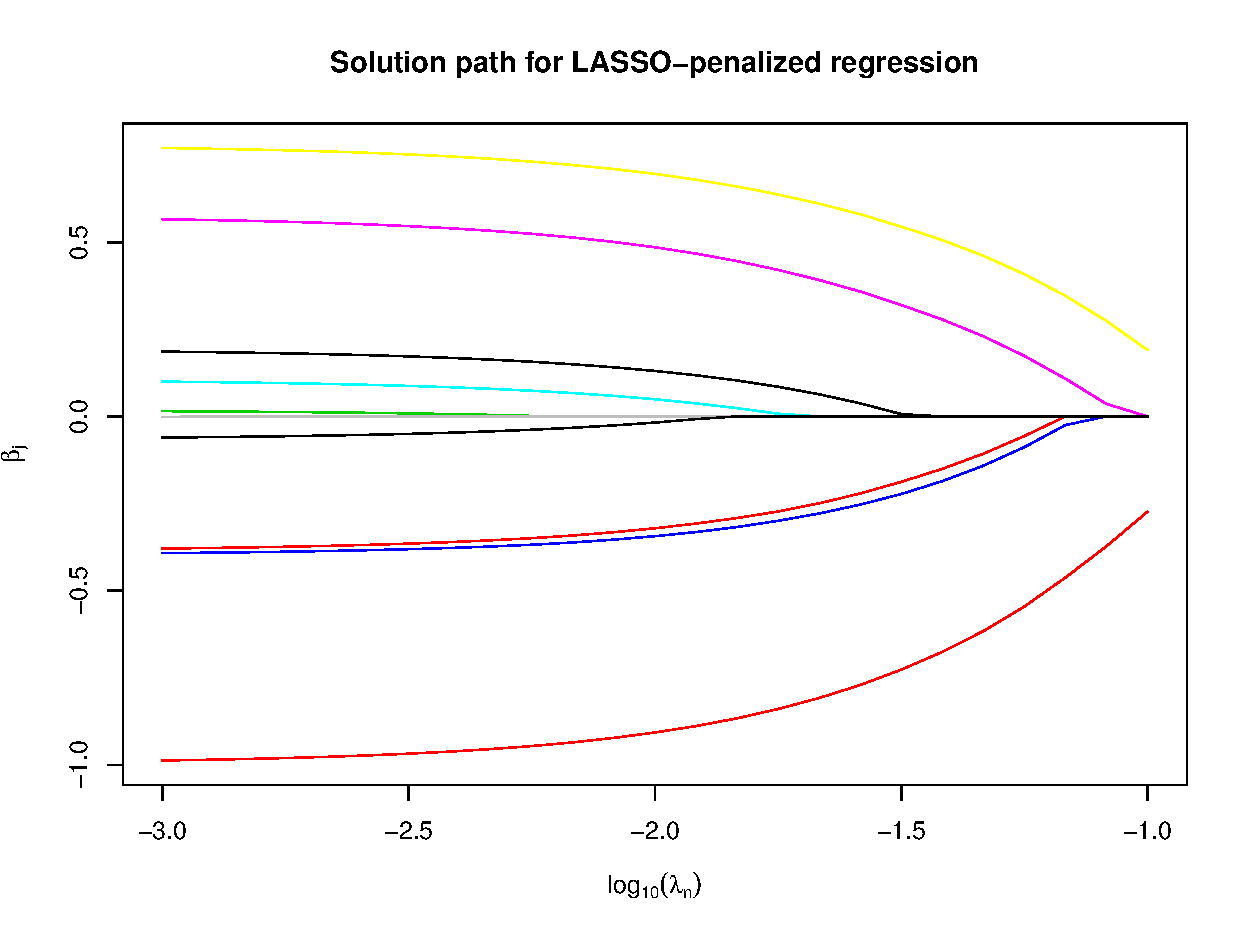
\includegraphics[scale = 0.6]{plots/new_LASSO-eps-converted-to.pdf}
\label{fig2:timing}
\caption{Path plot for LASSO-penalized Fine-Gray regression in our toy example.}
\end{figure}

\section{Simulation studies}
\label{s3:sim}
This section provides a more comprehensive illustration of the computational performance of the \CRANpkg{fastcmprsk} package over two popular competing packages \CRANpkg{cmprsk} and \CRANpkg{crrp}. 
We simulate datasets under various sample sizes and fix the number of covariates $p = 100$. We generate the design matrix, $\mathbf{Z}$
from a $p$-dimensional standard normal distribution with mean zero, unit variance, and pairwise correlation $\mbox{corr}(z_i, z_j) = \rho^{|i-j|}$, where $\rho = 0.5$ simulates moderate correlation. For Section \ref{s3:crr}, the vector of regression parameters for cause 1, the cause of interest, is $\bbeta_1 = (\bbeta^*, \bbeta^*, \ldots, \bbeta^*)$, where  $\bbeta^* = (0.40, -0.40, 0, -0.50, 0, 0.60, 0.75, 0, 0, -0.80)$. For Section \ref{s3:crrp}, $\bbeta_1 = (\bbeta^*, \mathbf{0}_{p - 10})$. We let $\bbeta_2 = -\bbeta_1$. We set $\pi =  0.5$, which corresponds to a cause 1 event rate of approximately $41\%$.  The average censoring percentage for our simulations varies between $30-35\%$.  We use  \code{simulateTwoCauseFineGrayModel} to simulate these data and average results over 100 Monte Carlo replicates. We report timing on a system with an Intel Core i5 2.9 GHz processor and 16GB of memory.

\subsection[Comparison to the crr package]{Comparison to the \CRANpkg{crr} package}
\label{s3:crr}
In this section, we compare the runtime and estimation performance of the \code{fastCrr} function to \code{crr}. We vary $n$ from $1000$ to $4000$ and run \code{fastCrr} and \code{crr} both with and without variance estimation. We take 100 bootstrap samples, {\color{blue}without parallelization}, to obtain the bootstrap standard errors with \code{fastCrr}. 

Figure 3 illustrates the runtime performance (in seconds) between both \code{fastCrr} (dashed lines) and \code{crr} (solid lines) as $n$ increases. It is clear that the performance of the \code{crr} methods increases quadratically while the \code{fastCrr} methods remain approximately linear. This leads to substantial improvement in computational performance for large sample sizes. Second, the forward-backward scan allows us to efficiently compute variance estimates through bootstrapping. We see that bootstrapping for smaller sample sizes may not result in computational gains; however, notable differences are observed for larger sample sizes. {\color{blue} Furthermore, since parallelization of the bootstrap procedure was not implemented in these timing reports, we expect multicore usage to further decrease the runtime of the variance estimation}. 

\begin{figure}[t!]
\centering
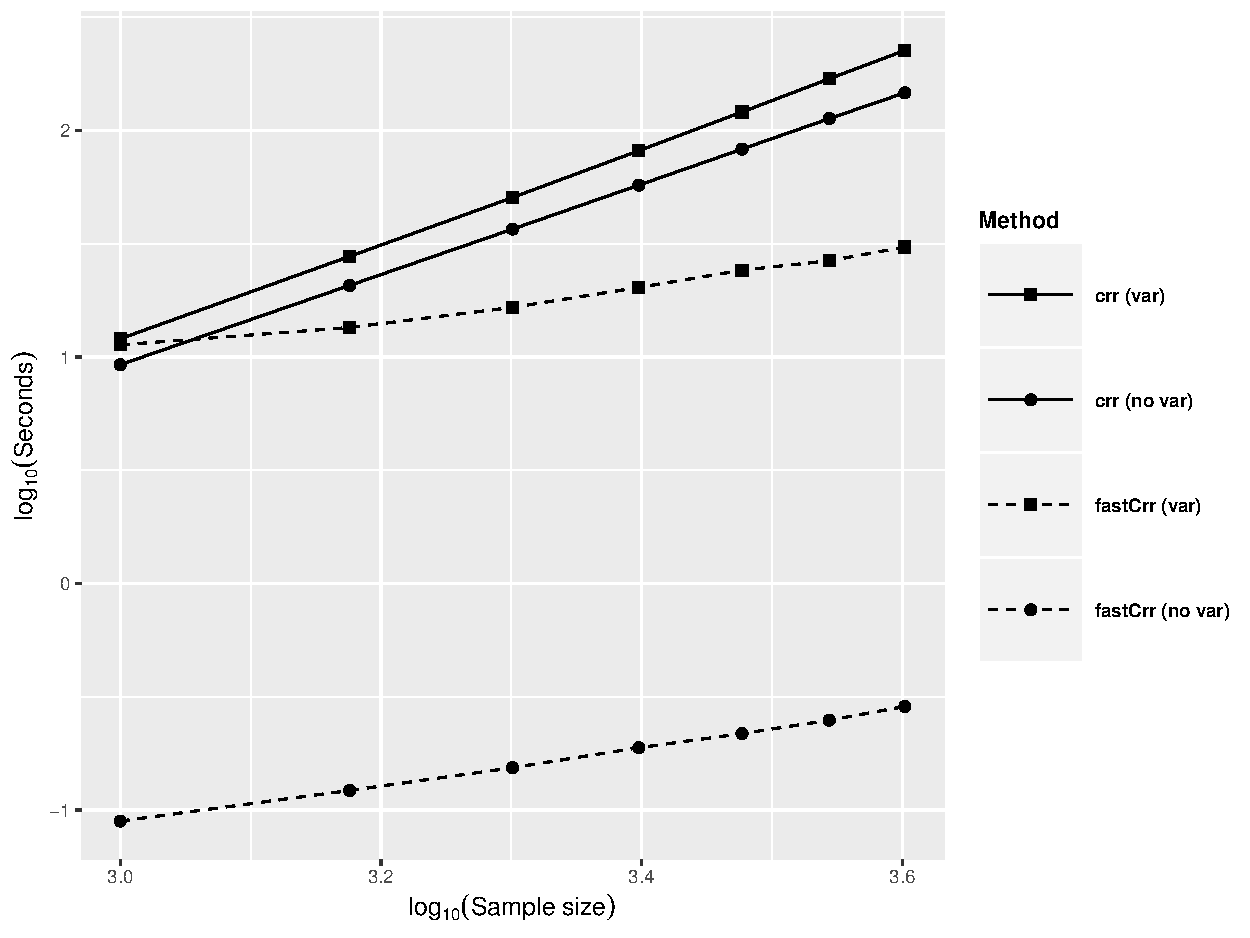
\includegraphics[scale = 0.6]{plots/log_NOPEN-eps-converted-to.pdf}
\label{fig3:timing}
\caption{Runtime comparison between \code{fastCrr} and \code{crr} with and without variance estimation.}
\end{figure}
To assess the performance of the bootstrap procedure for variance estimation, Table 3 shows the coverage probability (and standard errors) of the $95\%$ confidence intervals for $\bbeta_{11} = 0.4$.  We see  confidence intervals are generally wider for the bootstrap approach but are close to the nominal $95\%$ level.


\begin{table}[t!]
\centering
\setlength{\tabcolsep}{3.2pt}
\begin{tabular}{l|rrrr}
\toprule
  & $n$ = 1000  & 2000  & 3000 & 4000 \\ 
  \midrule
    \code{crr} & 0.93 (0.03) & 0.90 (0.03) & 0.93 (0.03) & 0.95 (0.02) \\ 
 \code{fastCrr} & 1.00 (0.00) & 0.96 (0.02) & 0.96 (0.02) & 0.96 (0.02) \\ 
   \bottomrule
\end{tabular}
\label{tab3:covprob}
\caption{Coverage probability (and standard errors) of $95\%$ confidence intervals for $\bbeta_{11} = 0.4$.}
\end{table}


\subsection[Comparison to the crrp package]{Comparison to the \CRANpkg{crrp} package}
\label{s3:crrp}
As mentioned in Section \ref{s3:pen}, \cite{fu2017penalized} provide an {R} package \CRANpkg{crrp} for performing penalized Fine-Gray regression using the LASSO, SCAD, and MCP penalties. We compare the runtime between \code{fastCrrp} with the implementation in the \CRANpkg{crrp} package. To level comparisons, we modify the source code in \code{crrp} so that the function only calculates the coefficient estimates and BIC score. We vary $n = 1000, 1500, \ldots, 4000$, fix $p = 100$,  and employ a  25-value grid search for the tuning parameter. Figure 4 illustrates the computational advantage the \code{fastCrrp}
function has over \code{crrp}. 

The computational performance of \code{crrp} (solid lines) increases quadratically while \code{fasrCrrp} (dashed lines) increases linearly, resulting in a 200 to 300-fold speed up in runtime when $n = 4000$. {\color{blue}This, along with the previous section, strongly suggests that for large-scale competing risks datasets (e.g. EHR databases), where the sample size can easily exceed tens to hundreds of thousands, analyses that may take several hours or days to perform using currently-implemented methods are available within seconds or minutes using our forward-backward scan algorithm.} 

\begin{figure}[t!]
\centering
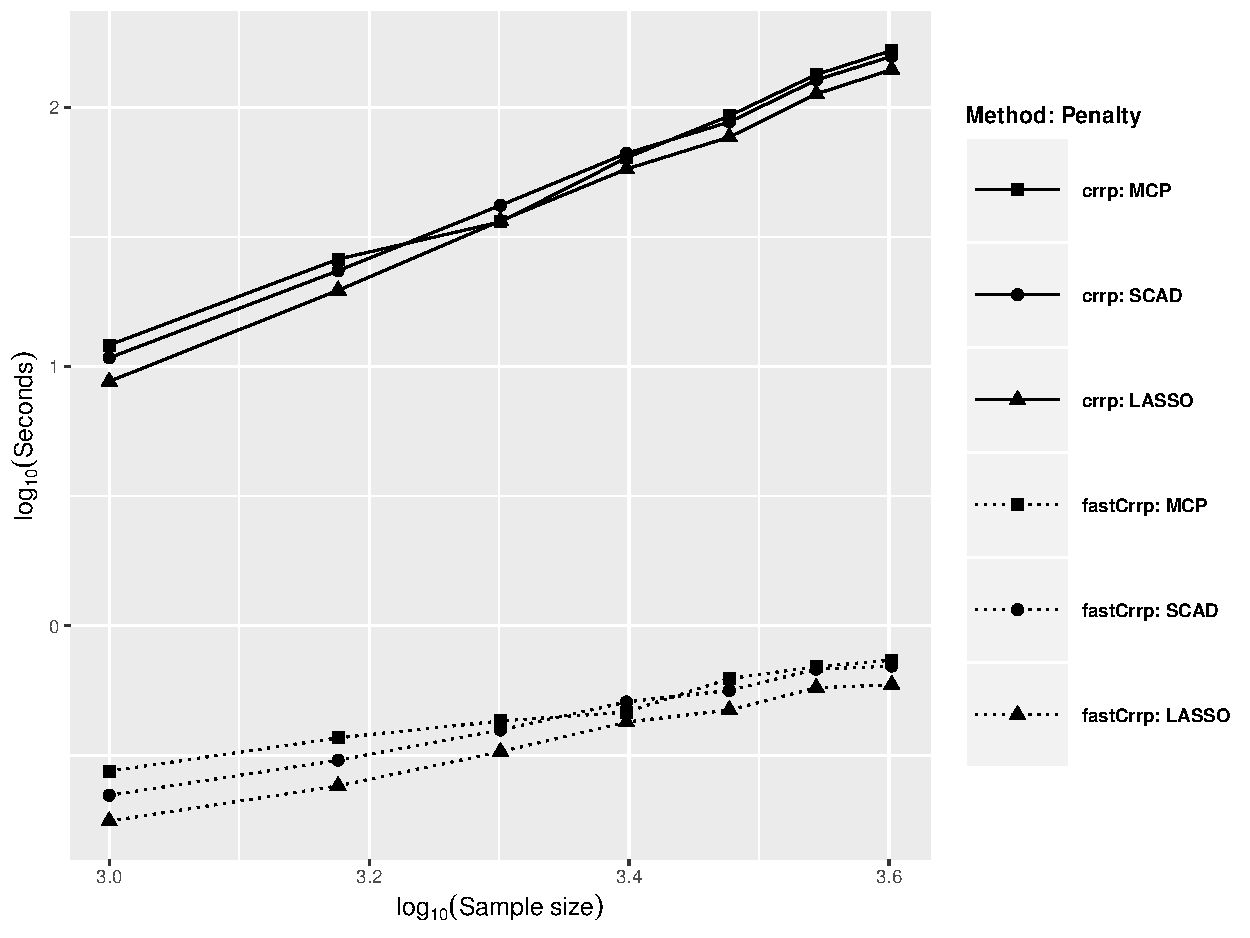
\includegraphics[scale = 0.6]{plots/log_PEN-eps-converted-to.pdf}
\label{fig3:pen}
\caption{Runtime comparison between the \CRANpkg{crrp} and \CRANpkg{fastcmprsk} implementations of LASSO, SCAD, and MCP penalization. Solid and dashed lines represent the \CRANpkg{crrp} and \CRANpkg{fastcmprsk} implementation, respectively. Square, circle, and triangle symbols denote the penalties MCP, SCAD, and LASSO, respectively.}
\end{figure}

\section{Discussion}
The \CRANpkg{fastcmprsk} package provides a set of scalable tools for the analysis of large-scale competing risks data by developing an approach to linearize the computational complexity required to estimate the parameters of the Fine-Gray proportional subdistribution hazards model. Multicore use is also implemented to further speed up methods that require bootstrapping and resampling. Our simulation results show that our implementation results in a 200-to-300 fold decrease in runtime for moderately large sample sizes. {\color{blue}In a real-world application, \cite{kawaguchi2019scalable} record an over 1000-fold decrease in runtime when comparing the forward-backward implementation to currently-available methods on a subset of the United States Renal Data Systems (USRDS) where $n =125, 000$, a sample size that is comparable to other EHR databases.} The package implements both penalized and unpenalized Fine-Gray regression. We can conveniently extend our forward-backward algorithm to other applications such as stratified and clustered Fine-Gray regression. 

Lastly, our current implementation assumes that covariates are densely observed across subjects. This is problematic in the sparse high-dimensional massive sample size (sHDMSS) domain \citep{mittal2013high} where the number of subjects and sparsely-represented covariates easily exceed tens of thousands. These sort of data are typical in large comparative effectiveness and drug safety studies using massive administrative claims and electronic health record (EHR) databases and typically contain millions to hundreds of millions of
patient records with tens of thousands patient attributes,
which such settings are particularly useful  for drug safety studies of a rare event such as unexpected adverse events 
\citep{schuemie2018improving} to protect public health. We are currently extending our algorithm to this domain in a sequel paper. 


\section{Acknowledgements}
{\color{blue} We thank the referees and the editor for their helpful comments that improved the presentation of the article}.
Marc A. Suchard's work is partially supported through the National Institute of Health grant U19 AI 135995. The research of Gang Li was partly supported by National Institute of Health Grants P30 CA-16042, UL1TR000124-02, and P50 CA211015.


%% -- Bibliography -------------------------------------------------------------
%% - References need to be provided in a .bib BibTeX database.
%% - All references should be made with \cite, \citet, \citep, \citealp etc.
%%   (and never hard-coded). See the FAQ for details.
%% - JSS-specific markup (, \CRANpkg, \code) should be used in the .bib.
%% - Titles in the .bib should be in title case.
%% - DOIs should be included where available.
%\bibliography{fastcmprsk}


%% -- Appendix (if any) --------------------------------------------------------
%% - After the bibliography with page break.
%% - With proper section titles and _not_ just "Appendix".

\newpage

\begin{appendix}

\section{Data generation scheme} 
\label{app3:data}
We describe the data generation process for the \code{simulateTwoCauseFineGrayModel} function. Let $n$, $p$, $\mathbf{Z}_{n \times p}$, $\bbeta_1$, $\bbeta_2$, $u\mbox{\tiny{min}}$, $u\mbox{\tiny{max}}$ and $\pi$ be specified. We first generate independent Bernoulli random variables to simulate the cause indicator $\ep$ for each subject. That is, $\ep_i \sim 1 + Bern\{(1 - \pi)^{\exp(\mathbf{z}_i^\prime \bbeta_1)}\}$ for $i = 1, \ldots, n$. Then, conditional on the cause, event times are simulated from 
\begin{align*}
\Pr(T_i \leq t | \ep_i = 1, \mathbf{z}_i) & = \frac{1 - [1 - \pi\{1 - \exp(-t)\}]^{\exp(\mathbf{z}_i^\prime\bbeta_1)}}{1 - (1 - \pi)^{\exp(\mathbf{z}_i^\prime\bbeta_1)}} \\
\Pr(T_i \leq t | \ep_i = 2, \mathbf{z}_i) & = 1 - \exp\{-t\exp(\mathbf{z}_i^\prime\bbeta_2)\}, \\
\end{align*}
and $C_i \sim U(u\mbox{\tiny{min}}, u\mbox{\tiny{max}})$. Therefore, for $i = 1, \ldots, n$, we can obtain the following quadruplet $\{(X_i, \delta_i, \delta_i \ep_i, \mathbf{z}_i)\}$ where $X_i = \min(T_i, C_i)$,  and $\delta_i = I(X_i \leq C_i)$. Below is an excerpt of the code used in \code{simulateTwoCauseFineGrayModel} to simulate the observed event times, cause and censoring indicators.

\begin{example}
#START CODE
...
...
...
# nobs, Z, p = pi, u.min, u.max, beta1 and beta2 are already defined.
# Simulate cause indicators here using a Bernoulli random variable
c.ind <- 1 + rbinom(nobs, 1, prob = (1 - p)^exp(Z %*% beta1))

ftime <- numeric(nobs)
eta1 <- Z[c.ind == 1, ] %*% beta1 #linear predictor for cause on interest
eta2 <- Z[c.ind == 2, ] %*% beta2 #linear predictor for competing risk

# Conditional on cause indicators, we simulate the model.
u1 <- runif(length(eta1))
t1 <- -log(1 - (1 - (1 - u1 * (1 - (1 - p)^exp(eta1)))^(1 / exp(eta1))) / p)
t2 <- rexp(length(eta2), rate = exp(eta2))
ci <- runif(nobs, min = u.min, max = u.max) # simulate censoring times

ftime[c.ind == 1] <- t1
ftime[c.ind == 2] <- t2 
ftime <- pmin(ftime, ci) # X = min(T, C)
fstatus <- ifelse(ftime == ci, 0, 1) # 0 if censored, 1 if event 
fstatus <- fstatus * c.ind  # 1 if cause 1, 2 if cause 2   
...
...
...            
\end{example}
\end{appendix}

\bibliography{kawaguchi}

\address{Eric S. Kawaguchi\\
  University of Southern California\\
  Division of Biostatistics and Epidemiology \\
  2001 N. Soto St. 
  Los Angeles, CA 90032, 
  USA\\
  \email{ekawaguc@usc.edu}}

\address{Jenny I. Shen \\
Los Angeles Biomedical Institute at Harbor-UCLA Medical Center \\
Division of Nephrology and Hypertension   \\
1124 W. Carson St. \\
Torrance, CA  90502,
 USA \\
  \email{jshen@labiomed.org}}

\address{Gang Li \\
University of California, Los Angeles\\
Department of Biostatistics \\
Los Angeles, CA 90095,
USA \\
  \email{vli@ucla.edu}}

\address{Marc A. Suchard\\
University of California, Los Angeles \\
Departments of Biostatistics, Biomathematics, and Human Genetics \\
Los Angeles, CA 90095,
USA \\
  \email{msuchard@ucla.edu}}